\documentclass[11pt]{article}                                                   
\usepackage[colorlinks]{hyperref}                                               
\usepackage{breakurl}                                                           
\usepackage{amsmath}                                                            
\usepackage[margin=.9in]{geometry}                                              
\newcommand{\nx}{\texttt{quigley}}                                              
\newcommand{\sechost}{\texttt{secureIpums}}                                     
\newcommand{\repo}{\texttt{/home/ipums-repo}}                                   
\newcommand{\ipums}{\texttt{$\sim$/IPUMS}}                                      
%\newcommand{\uP}{$\square$}                                                    
\newcommand{\ar}{$\rightarrow$}                                                 
\newcommand{\user}[1]{\texttt{#1}}                                              
\usepackage{mdframed}                                                           
%\usepackage{color}                                                             
%\usepackage{framed}                                                            
\usepackage{xcolor}       
\usepackage{graphicx}
\begin{document}

\title{The Rstudio175 cloud server\\
for Demog/Econ C175}

\maketitle
\tableofcontents

\section{Introduction}

The Rstudio175 cloud server is the computing infrastructure for all of the homework assignments in Demog/Econ 175. If you are not enrolled in this course, please hang up and dial 9-1-1.
\begin{mdframed}[backgroundcolor=blue!20]        
\textbf{There are two ways to use Rstudio}. We recommend using the \textbf{Rstudio175 Cloud Server} described below. However it is also possible to  to install the \textbf{Desktop} version of  Rstudio on your own machine and run program locally.

The Rstudio175 Cloud Server, will be maintained and supported so as to optimize your experience in Demography/Economics C175 and minimize your need to be your own system administrator.  If you like being your own sys/admin, and/or plan to work from a planet where there is no internet, the Desktop approach may suit you better\footnote{The indecisive can use both}. Just be aware that you're pretty much on your own with the Desktop version.  
\end{mdframed}
\section{Logging in to the Rstudio175 Cloud Server for the first time}

Shortly after registering for C175, you should receive email with instructions on how to initialize your account by setting your password.  All you should need to do is click on the link included in the email, and provide a new password.  If you never relieved this email verify that you are registered, then send email to trouble@demog.berkeley.edu.  Note that you must initialize your account within two weeks of the start of the semester to avoid administrative hurdles.

Once you have established a password for your Rstudio175 Cloud account, go to 
\url{http:courses.demog.berkeley.edu/goldsein175} and click on the large obvious button labeled ``Launch Rstudio175 Cloud'' to launch the Rstudio175 cloud.

You should soon be confronted with a web page sporting the Rstudio login dialog:

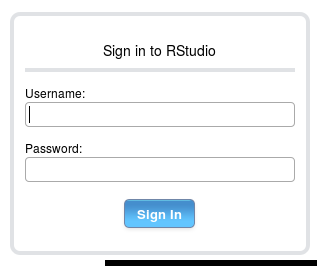
\includegraphics[scale=.35]{RstudioSignin}

Your username, (as indicated in the above mentioned email) is your
calnet ID (that is, the part of your @berkeley.edu email address that comes before the '@'. \textbf{but your password is whatever you set it to be}:
Rstudio175 uses an entirely separate password database from that of
Calnet.

\section{Some things to notice about Rstudio}

Once you have successfully given your Calnet ID and password, your browser window becomes a modern IDE\footnote{IDE stands for \emph{Integrated Development Environment} which means a computer program that helps you write computer programs.} IDEs are quite complicated programs used by professionals to make writing programs more efficient and less error prone.

You will use only a small fraction of the features of Rstudio -- but should you (wisely) go on to master R, you will come to be amazed at the cleverness of this thing. Unfortunately,  before amazement comes bewilderment at the number of features present.

Your initial Rstudio window should look something like this:

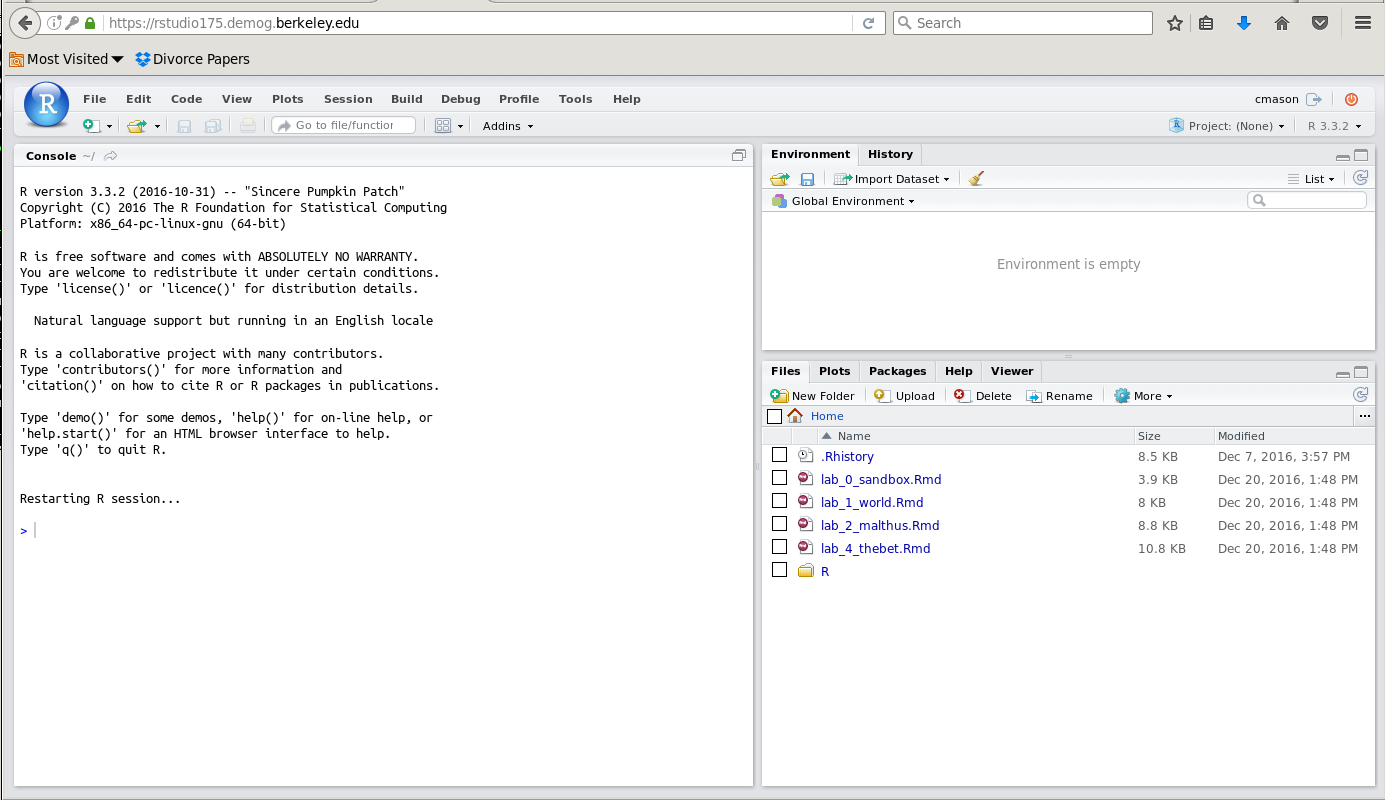
\includegraphics[scale=.35]{RstudioStart}

\textbf{BEFORE touching anything} Please Notice the following:

\begin{itemize}
\item The left hand pane, labeled ``console''  is an R interpreter.  It will take and process R commands such as you have already learned from assigned R instructions [insert clearer description here of what students were supposed to do to learn R]

\item The lower right hand pane should hold the file viewer. If it does not look like the picture above, then make sure the ``Files'' tab is depressed.

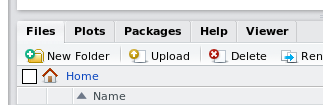
\includegraphics[scale=.5]{RstudioFiles}

The file viewer gives you access to your files.  You should have several files with names like 'lab\_0\_sandbox.Rmd' or 'lab\_4\_thebet.Rmd'.   These are your weekly homework assignments.  The files download automatically \textbf{if you directory does not already contain a file with the same name}.  This means that if, while working on one of your assignments, you decide to declare bankruptcy and start over, you can simply delete or rename the file (check the box and hit the delete or rename button) then log out and log back in and a fresh copy of the file will be there.

\item To work on a homework assignment, simply click on the blue hypertext file name

\includegraphics[scale=.5]{RstudioHyplink} and behold:  the \emph{Console} pane will shrink to a little nothing at the bottom of the window and its former place will be filled with an ``R notebook''.

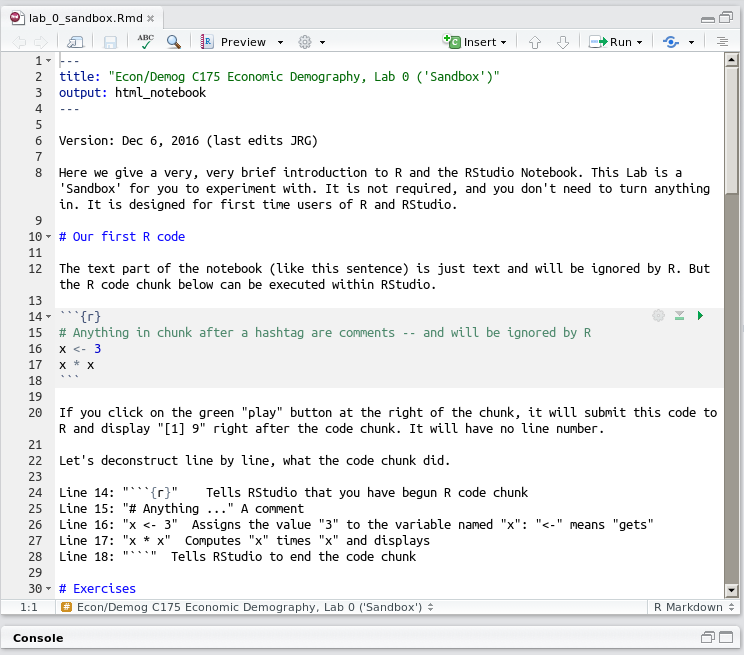
\includegraphics[scale=.3]{RstudioRnotebook}


\end{itemize}

\section{Working in Rstudio}

The majority of your work should be within the ``R notebook''.  That is, most of what you will do for homework will be to read the instructions (in the r notebook); then execute some code; then change the code and execute it again.

The purpose of the code is to learn. Once you have learned what you can from the code, you will go to Bcourses and answer the questions at the end of each R notebook.   

\subsection{Executing code chunks}

In the R notebook, code comes in ``chunks'' interspersed with regular text such as this.  The code chunks look like this:

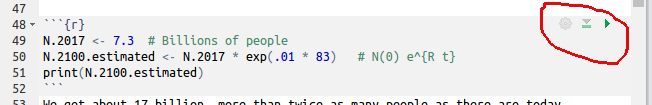
\includegraphics[scale=.5]{RstudioChunk}

They are set off from the text by a light gray background and have three buttons in their upper right corner.  The green triangle on the far right is the most useful, it executes the code \textbf{in the current block only}. You'll generally want to use this button after making changes to the code chunk.

\subsection{Checking your work}

In order to keep you from going off the rails, each notebook contains a few special code chunks which are designed to check your work. This is not for grading purposes, but rather to let you know that you are doing things right.

The special code chunks look and function the same way other code chunks function-- you make changes to the code then execute it by hitting the greed triangle.

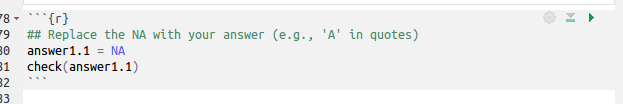
\includegraphics[scale=.5]{RstudioCheck}

The difference is that these code chunks expect you to change only the line that assigns a value to a variable called \textbf{answer1.1} (1.1 will of course change).  After specifying the answer and running the code chunk, you will receive either a dopamine rich message of congratulations, or encouraging hint.  You may execute these chunks as many times as you wish. Their purpose is to help you --not to judge you.


\end{document}

%  LocalWords:  Rstudio edu IDE IDEs Rmd Bcourses
